% THIS IS AN EXAMPLE DOCUMENT FOR VLDB 2012
% based on ACM SIGPROC-SP.TEX VERSION 2.7
% Modified by  Gerald Weber <gerald@cs.auckland.ac.nz>
% Removed the requirement to include *bbl file in here. (AhmetSacan, Sep2012)
% Fixed the equation on page 3 to prevent line overflow. (AhmetSacan, Sep2012)

\documentclass[]{vldb}

\usepackage{graphicx}
\usepackage{balance}  % for  \balance command ON LAST PAGE  (only there!)
\usepackage{url}
\usepackage{hyperref}
\usepackage{microtype}
\usepackage{calc}
\usepackage[final]{listings}
\usepackage[table]{xcolor}
\usepackage{xcolor}
\usepackage[utf8]{inputenc}
\usepackage{upquote}
\usepackage{fixme}
\usepackage{xfrac}
\usepackage{minted}
\usepackage{amsmath,amssymb}
\usepackage{siunitx}
\usepackage{subfig}
\usepackage{pmboxdraw} % Dark boxes for text histograms
\usepackage{array,multirow}
\usepackage{tikz}
\usepackage{xspace}
\usetikzlibrary{patterns}
\makeatletter
\global\let\tikz@ensure@dollar@catcode=\relax
\makeatother

\fxsetup{nomargin,inline}

% Images in draft mode
\setkeys{Gin}{draft=false}

\newlength{\barlength}

\newcommand{\singlebar}[1]{
  \setlength{\barlength}{\dimexpr #1em / 2 \relax}
  \begin{tikzpicture}
    \draw[pattern=north east lines,pattern color=.] (0,0) rectangle (\barlength,0.5em);
  \end{tikzpicture}
}

\lstset{ %
  basicstyle=\ttfamily\small\color{black},  %
  breaklines=true, %
  keywordstyle=\textbf, %
  literate={█}{{\singlebar{1}}}{1}
           {██}{{\singlebar{2}}}{2}
           {███}{{\singlebar{3}}}{3}
           {████}{{\singlebar{4}}}{4}
           {█████}{{\singlebar{5}}}{5}
           {██████}{{\singlebar{6}}}{6}
           {███████}{{\singlebar{7}}}{7}
           {████████}{{\singlebar{8}}}{8}
           {█████████}{{\singlebar{9}}}{9}
           {██████████}{{\singlebar{10}}}{10}
           {███████████}{{\singlebar{11}}}{11}
           {████████████}{{\singlebar{12}}}{12}
           {█████████████}{{\singlebar{13}}}{13}
           {██████████████}{{\singlebar{14}}}{14}
           {███████████████}{{\singlebar{15}}}{15}
           {████████████████}{{\singlebar{16}}}{16}
           {█████████████████}{{\singlebar{17}}}{17}
           {██████████████████}{{\singlebar{18}}}{18}
           {███████████████████}{{\singlebar{19}}}{19}
           {████████████████████}{{\singlebar{20}}}{20}
           {█████████████████████}{{\singlebar{21}}}{21}
           {██████████████████████}{{\singlebar{22}}}{22}
           {███████████████████████}{{\singlebar{23}}}{23}
           {████████████████████████}{{\singlebar{24}}}{24}
           {█████████████████████████}{{\singlebar{25}}}{25}
           {▌}{{\singlebar{0.5}\hspace{\dimexpr0.5em-0.5em/2\relax}}}{1}
           {•}{{$\bullet$}}{1},
  moredelim=[is][\color{red}\underbar]{\$}{\$}, %
  moredelim=[is][\color{red}]{/}{/}, %
  upquote=true, %
  keepspaces=true, %
  basewidth=0.5em %
}

\lstnewenvironment{lstnobreak}[1][]
{\noindent\minipage{\linewidth}\medskip\lstset{#1}}
{\endminipage}

\hypersetup{breaklinks=true,
            bookmarks=true,
            pdfauthor={},
            pdftitle={},
            colorlinks=true,
            citecolor=blue,
            urlcolor=blue,
            linkcolor=magenta,
            pdfborder={0 0 0}}

\DeclareMathOperator{\Var}{Var}
\DeclareMathOperator{\Covar}{Covar}

\newlength{\figurepadding}
\setlength{\figurepadding}{0.5em}
\newcommand{\paddedgraphics}[2][]{\includegraphics[#1]{#2}\vspace{\figurepadding}}
\newcommand{\timing}[4][\second]{analysis time: \SI{#2}{#1}, training time: \SI{#3}{\second}, total runtime: \SI{#4}{#1}}

\def\dBoost/{\emph{dBoost}\xspace}

\newcommand{\srm}[1]{\textcolor{red}{Sam: {#1}}}
\newcommand{\cpc}[1]{\textcolor{blue}{Clément: {#1}}}

% Local Variables:
% mode: latex
% End:


\begin{document}

% ****************** TITLE ****************************************

% TODO: "dBoost: " User-Guided
%\title{User-Guided Outlier Detection in Heterogeneous Datasets}
\title{Outlier Detection in Heterogeneous Datasets using Automatic Tuple Expansion}

% ****************** AUTHORS **************************************

% You need the command \numberofauthors to handle the 'placement
% and alignment' of the authors beneath the title.
%
% For aesthetic reasons, we recommend 'three authors at a time'
% i.e. three 'name/affiliation blocks' be placed beneath the title.
%
% NOTE: You are NOT restricted in how many 'rows' of
% "name/affiliations" may appear. We just ask that you restrict
% the number of 'columns' to three.
%
% Because of the available 'opening page real-estate'
% we ask you to refrain from putting more than six authors
% (two rows with three columns) beneath the article title.
% More than six makes the first-page appear very cluttered indeed.
%
% Use the \alignauthor commands to handle the names
% and affiliations for an 'aesthetic maximum' of six authors.
% Add names, affiliations, addresses for
% the seventh etc. author(s) as the argument for the
% \additionalauthors command.
% These 'additional authors' will be output/set for you
% without further effort on your part as the last section in
% the body of your article BEFORE References or any Appendices.


\newcommand{\MITauthor}[2]{#1\\\affaddr{MIT CSAIL}\\\email{#2@mit.edu}}
\newcommand{\CSAILauthor}[2]{#1\\\affaddr{MIT CSAIL}\\\email{#2@csail.mit.edu}}

\numberofauthors{3}
\author{
  \alignauthor\MITauthor{Clément Pit-\kern0pt-Claudel}{cpitcla} 
  \alignauthor\MITauthor{Zelda Mariet}{zmariet} \\\vspace{0.2in} \CSAILauthor{Sam Madden}{madden}
  \alignauthor\MITauthor{Rachael Harding}{rhardin} 
}

\date{10 December 2014} %TODO

\maketitle

\begin{abstract}
Rapidly developing areas of information technology are generating massive amounts of data. Human errors, sensor failures, and other unforeseen circumstances unfortunately tend to undermine the quality and consistency of these datasets by introducing outliers -- data points that exhibit surprising behavior when compared to the rest of the data. Characterizing, locating, and in some cases eliminating these outliers offers interesting insight about the data under scrutiny and reinforces the confidence that one may have in conclusions drawn from otherwise noisy datasets.

In this paper, we describe a new user-guided outlier detection framework, \dBoost, which relies on inference and statistical modeling of heterogeneous data to flag suspicious fields in database tuples. At the heart of the system lies a tuple expansion procedure, which reconstructs rich information from semantically poor SQL data types such as strings, integers, and floating point numbers. We show that this novel approach achieves good classification performance, both in traditional numerical datasets and in highly non-numerical contexts such as mostly textual datasets. Our implementation is publicly available, under version 3 of the GNU General Public License.
\end{abstract}


\section{Introduction}
\label{sec:intro}

Sensor glitches, data-entry errors, and malicious activities are a few examples of events that can lead to the appearance of outliers in a dataset. If undetected, these values can skew statistics, support invalid conclusions, slow database operations, and cause otherwise avoidable expenses. On the other hand, careful analysis of these values can yield new insight about the data, prevent undesirable events, and generally improve the reliability of the data~\cite{Achour2014}.

Previous literature has generally defined an outlier as ``an observation which deviates so much from the other observations as to arouse suspicions that it was generated by a different mechanism'' \cite{Hawkins1980}, and has suggested a number of ways to detect and in some cases eliminate suspicious values. Previous approaches to outlier detection include modeling numerical data using Gaussian Mixture Models~\cite{Lu2005,Roberts1994,Roberts1999}, Histogram modeling~\cite{Gebski2007,Sheng2007}, and $k$-nearest neighbors~\cite{Ramaswamy2000}.

Little work, however, has focused on developing generic methods for user-guided outlier detection that work with widely diverse and heterogeneous data stored in typical relational database management systems. The relative inexpressivity of basic SQL types -- integers, strings, and doubles in particular -- might be to blame: strings, for example, can be used to store information as diverse as city names, email addresses, or phone numbers; typically it is the job of application logic to encode the semantically rich domains of these values as one of the basic SQL data types. This paucity of semantic information leaves outlier detection algorithms that run inside of the database with very little information to work with.

This paper presents a new approach for detecting outliers in highly heterogeneous datasets: our tools systematically expand the limited space of SQL types to derive richer information.
This is done automatically, by applying a library of possible transformations (which we call ``expansions'') to the values of each column in a table to find rules that are consistent with the bulk of the values that appear in the column.
For example, integers can expanded into dates and times by considering them as Unix timestamps, and into sets of booleans by considering them as bit vectors.
If an expansion of an integer column to a the day of week from a date found that most of the dates reconstructed from an integer column fall on the same day of the week, then values falling on other days might be flagged as suspicious.
As in this example, these expansions  can be used to detect outliers that are difficult or impossible to detect using raw data and provide detailed reports to the user.

Hence, our main contribution is a method that automatically applies expansion rules (type-dependent transformations) to create a set of derived attributes for every tuple. These derived attributes are then processed by several outlier detection models to efficiently learn soft constraints about the individual attributes, and to detect soft functional dependencies \textit{between} derived attributes, enabling multidimensional models to detect of a broad class of data inconsistencies. By extracting numerical or highly structured attributes from unstructured data (for example, by extracting casing information from strings), our method makes it significantly easier to detect inconsistencies that would have escaped sophisticated outlier detection systems.

We designed our system to be both fast and memory efficient; it proceeds in three online passes over the data, keeping no more information than strictly necessary (in general, no more than a few dozen values per field in the database schema). The architecture is parallelizable, the analysis can be distributed over multiple computation nodes, and information can be kept from one run to the next so as to eliminate the first and possibly the second pass.

In summary, our contributions are as follows:
\begin{enumerate}
\item We present the concept of tuple expansion, a method used to reconstruct structured and semantically rich information from raw database data using a user-extensible library of type-dependent expansion rules, and we describe a library of broadly applicable expansion rules that have proven useful for flagging outliers in heterogeneous datasets.
\item We show that these expansions can be fed to both single and multi-variate models to accurately detect outliers without making strong assumptions about the original data\footnote{For example, we do not restrict the types used to store the data: we are able to find outliers in textual data}. In addition to typical Gaussian modeling strategies, we present a metric used to detect outlying values on histograms, and a novel combination of attribute-based partitioning and modeling.
\item We demonstrate on several synthetic and real-world datasets (including numerical and non-numerical data and homo- and heterogeneous datasets) that simple, well-known statistical models are enough to detect many data inconsistencies once tuple expansion has been applied, whereas these inconsistencies would have remained hidden without tuple expansion.
\end{enumerate}

The rest of this paper is structured as follows: In Section~\ref{sec:overview} we present an overview in the framework. We then detail our tuple expansion method in Section~\ref{sec:expansion}, before applying it to outlier detection in Section~\ref{sec:implementation}. We evaluate our tool on synthetic and real-world datasets in Section~\ref{sec:evaluation}, and we describe related work in Section~\ref{sec:related-work}. Finally, we conclude in Section~\ref{sec:conclusion}. % TODO \item We outline directions for future work in Section~\ref{sec:future-work}.

\section{Outlier Detection Engine}
\label{sec:implementation}
Each tuple is extended with all of the possible expansions of all of its fields.
These expanded tuples are fed into the statistical analyzer, which looks at the distribution of values in each expanded column and identifies tuples with expanded attribute values, or pairs of attribute values, that are outliers.
\section{Overview of dBoost}
\label{sec:overview}

We designed a framework that analyzes, models, and detects outliers in data.
The whole system can be seen in Figure~\ref{fig:pipeline}.

\begin{figure*}
  \centering %TODO: Should this be full width?
  \paddedgraphics[width=.8\textwidth]{../graphics/pipeline.pdf}
  \caption{Framework pipeline}
  \label{fig:pipeline}
\end{figure*}

As a first step, tuples are read from the database and expanded: a set of type-dependent features is extracted for each field. These features express simple properties of the data, such as the length of a string, or the parity of an integer.

These expanded tuples are then analyzed in order to obtain simple statistical information, and to detect soft functional dependencies between different fields. The expanded tuples are then used to train one of three data models, with the help of the  statistics and correlation hints gathered at the previous stage.

Finally, the trained model is used to classify tuples into regular records and outliers; these tuples can be the ones the model was trained with, or future inputs to the database system.

From a high level view, our pipeline is implemented as a three-pass streaming algorithm, requiring no memory beyond that required to train the individual models.

The different stages of our pipeline are summarized as follows and described in detail in the following sections:

\begin{enumerate}
\item Preprocessing -- Tuples are expanded using knowledge about the database schema and field types (Section~\ref{sec:preprocessing}).
\item Statistical analysis -- The expanded data is analysed to gather basic statistics, along with correlation information. These statistics are used for modeling and outlier detection (Section~\ref{sec:statistical-analysis}).
\item Data modeling -- We apply various user-selected machine-learning algorithms to build models of the data (Section~\ref{sec:model-creation}).
\item Outlier detection -- Using the models built in the previous stage and user-provided sensitivity thresholds, we report outliers identified by the models trained during the previous stage (Section~\ref{sec:outlier-detection}).
\end{enumerate}

\section{Tuple Expansion}
\label{sec:expansion}

\vspace{0.1in}

\noindent
\begin{minipage}{\linewidth}
  \begin{minipage}{0.8\linewidth}
    \itshape
    What if you need to store a date and time value with subsecond resolution? MySQL
    currently does not have an appropriate data type for this, but you can use your own
    storage format: you can use the BIGINT data type and store the value as a timestamp in
    microseconds, or you can use a DOUBLE and store the fractional part of the second after
    the decimal point.
  \end{minipage}
  \begin{flushright}
    \textit{High-Performance MySQL}, 3\textsuperscript{rd} edition (2012), p.~127
  \end{flushright}
\end{minipage}\vspace{\figurepadding}

Data stored in databases often has rich semantics, encompassing dates and times, highly stuctured datatypes such as phone numbers, addresses, or GIS data. The semantics of plain SQL, however, are not expressive enough to properly store these rich data types. Programmers are thus forced to revert to simpler types, relying on application logic to parse the data.  
\srm{Note that users of databases have user-defined types, but that these often are not used.}

Unfortunately, structural information on the data is what tasks such as outlier detection would most benefit from. For example, the day of the week in a date may be relevant information in a banking application in which transactions are only completed on weekdays, but unless the programmer explicitly duplicates this information in a separate column, it remains inaccessible to an automated outlier detector.

\srm{I think we should present the library as more of a contribution, i.e., ``Our tool comes with a large library of such features we have found useful in several different applications we have applied our tool to.''}
To reconstruct this lost information we expand tuples, expanding each field with sub-tuples of extracted type-depent features based on the data type of the field.
The rules by which tuples are expanded are taken from a library provided with our tool.
Figure~\ref{fig:tuple-expansion} lists some of the rules our library provides for three common data types. These rules serve as a starting point for tuple expansion, but we expect users of our toolbox to expand this set of rules to add insight specific to their application domain. Expressing rules as simple functions mapping a value of a given type to a tuple of features makes it possible to express soft constraints about the data easily: instead of specifying hard constraints, users state that a certain way of looking at attributes should be consistent across the rows of the table. 

\newenvironment{stackedlines}{\renewcommand{\arraystretch}{1.2}\begin{array}[b]{@{}l@{\quad}l@{}}}{\end{array}}
\newcommand{\sigrule}[1]{\mbox{\texttt{\spaceskip=0.1em{#1}}}}

\begin{figure}[h]
  \newcommand{\largest}{date, \ldots:}
  $\begin{stackedlines}
    \texttt{string:}\\
    \texttt{\parbox{\widthof{1418222134.325}}{"32-G414"}}
  \end{stackedlines} \rightarrow
  \begin{cases}
    % \text{id:} & \texttt{32-G414}\\
    \text{length:} & \texttt{7}\\
    \text{signature:} & \sigrule{Nd Nd Pd Lu Nd Nd Nd}\\
    \text{uppercase:} & \texttt{True (1)}\\
    \text{lowercase:} & \texttt{False (0)}\\
    \text{email ok:} & \texttt{False (0)}\\
    \text{stripped:} & \texttt{<num>-G<num>}\\
    \text{\parbox{\widthof{\largest}}{title case:}} & \texttt{True (1)}
  \end{cases}\hfill$
% \end{figure}
% \begin{figure}[H]
  $\begin{stackedlines}
    \texttt{int:}\\
    \texttt{\parbox{\widthof{1418222134.325}}{1418222134}}
  \end{stackedlines} \rightarrow
  \begin{cases}
    % \text{id:} & \texttt{1418222134}\\
    \text{date:} & \texttt{(2014,12,10)}\\
    \text{time:} & \texttt{(14,35)}\\
    \text{weekday:} & \texttt{Wed (2)}\\
    % \text{day of year:} & \texttt{344}\\
    \text{weekend:} & \texttt{False (0)}\\
    \text{binary:} & \texttt{0b10101\ldots010}\\
    \text{\parbox{\widthof{\largest}}{mod-10:}} & \texttt{4}
  \end{cases}\hfill$
% \end{figure}
% \begin{figure}[H]
   $\begin{stackedlines}
    \texttt{float:}\\
    \texttt{1418222134.325}
  \end{stackedlines} \rightarrow
  \begin{cases}
    % \text{id:} & \texttt{1418222134.325}\\
    \text{intpart:} & \texttt{1418222134}\\
    \text{fracpart:} & \texttt{0.325}\\
    \text{millis:} & \texttt{325}\\
    \text{\parbox{\widthof{\largest}}{date, \ldots:}} & \texttt{\ldots}
  \end{cases}\hfill$

  \caption{Selected tuple expansion rules.}
  \label{fig:tuple-expansion}
\end{figure}

The rules presented in Figure~\ref{fig:tuple-expansion} are fairly general rules, likely to apply to be suitable to most datasets For example, the \texttt{strip numbers} rule takes a string, and replaces any sequence of digits by the string \texttt{<num>}. Such a rule is useful to check that a column is formatted consistently, allowing for variations only in the numbers: a database of legislative citations, for example, could contain entries such as \texttt{S.933}, \texttt{H.R.21}, \texttt{P.L.107-155}, or \texttt{P.L.88-352}; applying the \texttt{strip numbers} rule to this data yields \texttt{S.<num>}, \texttt{H.R.<num>}, \texttt{P.L.<num>-<num>}, or \texttt{P.L.<num>-<num>}; this reduces the whole dataset to a small number of patterns that can be easily analyzed using data models.

The \texttt{signature} rule is equally interesting: to extract the signature of a string, our tools replace each character by the name of its Unicode class: uppercase Latin letters are \texttt{Lu}, lowercase Latin letters are \texttt{Ll}, digits are \texttt{Nd}, and punctuation signs are among others \texttt{Po}, \texttt{Pe}, \texttt{Ps}, and \texttt{Pd}. Such a rule is useful to check the consistency of various fixed-width formats such as ISO~8061 timestamps, birth dates, or phone numbers. As a more detailed example, a column in a database could be used to record references to particular sections, subsections, and paragraphs in a text: entries would be in the form \texttt{\S901.04(a)}, \texttt{\S853.02(d)}, or \texttt{\S910.45}. Extracting the signature of these entries would yield \sigrule{Po Nd Nd Nd Po Nd Nd Ps Ll Pe} for the first two entries, and \sigrule{Po Nd Nd Nd Po Nd Nd} for the last one. Just like before, this reduces the dataset to a small set of patterns, making it easy to detect discrepancies. %TODO Cite unicode standard

%\subsection{Preprocessing}
\label{sec:preprocessing}

Before being used to generate a model of the data, the tuples are expanded in order to reveal and extract potentially relevant information.

\subsubsection{Tuple Expansion}

\noindent
\begin{minipage}{\linewidth}
  \begin{minipage}{0.8\linewidth}
    \itshape
    What if you need to store a date and time value with subsecond resolution? MySQL
    currently does not have an appropriate data type for this, but you can use your own
    storage format: you can use the BIGINT data type and store the value as a timestamp in
    microseconds, or you can use a DOUBLE and store the fractional part of the second after
    the decimal point.
  \end{minipage}
  \begin{flushright}
    \textit{High-Performance MySQL}, 3\textsuperscript{rd} edition (2012), p.~127
  \end{flushright}
\end{minipage}\vspace{\figurepadding}

Data stored in databases often has rich semantics, encompassing dates and times, highly stuctured datatypes such as phone numbers or addresses, or GIS data. The semantics of plain SQL, however, are not expressive enough to properly store these rich data types. Programmers are thus forced to revert to simpler types, relying on application logic to parse the data.

Unfortunately, information on the structure of this data is also what an outlier detection engine would most benefit from. For example, the day of the week in a date may be relevant information in a banking application in which transactions are only completed on weekdays, but unless the programmer explicitly duplicates this information in a separate column, it remains inaccessible to an automated outlier detector.

To reconstruct potentially lost information we expand tuples, breaking down each field into a sub-tuple of extracted type-depent features. Figure~\ref{fig:tuple-expansion} lists the rules that we apply to values of these three data types. These rules serve as a starting point for tuple expansion, but we expect users of our toolbox to expand this set of rules to add insight specific to their application domain. Expressing rules as simple functions mapping a value of a given type to a tuple of features makes it possible to express soft constraints about the data easily: instead of specifying hard constraints, users state that a certain way of looking at the data should consistent across the rows of the table.

\newenvironment{stackedlines}{\renewcommand{\arraystretch}{1.2}\begin{array}[b]{@{}l@{\quad}l@{}}}{\end{array}}

% todo: Merge figures?
\begin{figure}[H]
  $\begin{stackedlines}
    \texttt{string:}\\
    \texttt{\parbox{\widthof{1418222134.325}}{"32-G414"}}
  \end{stackedlines} \longrightarrow
  \begin{cases}
    \text{id: } & \texttt{32-G414}\\
    \text{length: } & \texttt{7}\\
    \text{signature: } & \texttt{NNPLNNN}\\
    \text{uppercase: } & \texttt{True (1)}\\
    \text{lowercase: } & \texttt{False (0)}\\
    \text{valid email: } & \texttt{False (0)}\\
    \text{erase numbers: } & \texttt{<num>-G<num>}\\
    \text{\parbox{\widthof{base-10 residue:}}{title case:} } & \texttt{True (1)}
  \end{cases}$
% \end{figure}
% \begin{figure}[H]
  $\begin{stackedlines}
    \texttt{int:}\\
    \texttt{\parbox{\widthof{1418222134.325}}{1418222134}}
  \end{stackedlines} \longrightarrow
  \begin{cases}
    \text{id: } & \texttt{1418222134}\\
    \text{date: } & \texttt{(2014,12,10)}\\
    \text{time: } & \texttt{(14,35)}\\
    \text{weekday: } & \texttt{Wed (2)}\\
    \text{day of year: } & \texttt{344}\\
    \text{weekend: } & \texttt{False (0)}\\
    \text{binary: } & \texttt{0b10101\ldots010}\\
    \text{mod-10 residue: } & \texttt{4}
  \end{cases}$
% \end{figure}
% \begin{figure}[H]
   $\begin{stackedlines}
    \texttt{float:}\\
    \texttt{1418222134.325}
  \end{stackedlines} \longrightarrow
  \begin{cases}
    \text{id: } & \texttt{1418222134.325}\\
    \text{intpart: } & \texttt{1418222134}\\
    \text{fracpart: } & \texttt{0.325}\\
    \text{millis: } & \texttt{325}\\
    \text{\parbox{\widthof{base-10 residue:}}{date, \ldots:} } & \texttt{\ldots}
  \end{cases}$

  \caption{Selected tuple expansion rules.}
  \label{fig:tuple-expansion}
\end{figure}
\subsection{Statistical Analysis}
\label{sec:statistical-analysis}

Following the tuple expansion phase, the expanded tuples go through the statistical analysis phase. This phase collects simple statistics on each column of the table, and estimates which sets of columns are correlated.

The statistical information includes the average, variance, standard deviation and extremes of each numerical column, as well as approximate cardinality measurements for all columns. These statistics have two purposes. First, they are used at the end of the statistical analysis phase to determine which columns in the table are correlated. Second, the statistics can be used during data modeling to speed up the training phase of certain models by precompiling parameters needed by the models (e.g., mean and standard deviation for the Gaussian model).

We focus on two inter-column correlation detection strategies:

\begin{itemize}
\item For mostly-numeric datasets, we use Pearson's product-moment
  correlation. It relies on the Pearson correlation coefficient,
  which measures linear dependencies between two vectors.

  Given two column vectors $X$ and $Y$, Pearson's coefficient $R$ is given by the following formula:
  \begin{align}
    \label{eqn:pearson}
    R = \frac{\Covar(X,Y)}{\sqrt{\Var(X)\Var(Y)}}
  \end{align}

  $R$'s value always lies between $-1$ and $1$. An $R$ value close to 0 indicates little or no correlation, while values close to $+1$ or $-1$ indicate strong positive or negative correlations, respectively. Pairs of columns with a value of \(R\) above a user-specified threshold are added to a list of correlation hints, for use by the models.

\item For mostly non-numeric datasets, we use a cardinality-based measure, flagging groups of expanded columns as correlated when their joint cardinality is below a user-specified threshold. This works well, because when two columns are correlated (for example, when one is computed from the other) the number of distinct pairs in the columns is roughly the same as the number of distinct items in any of them; on the other hand, when two columns are independent, the number of distinct pairs is close to the product of the number of distinct values in each column).
\end{itemize}

It is debatable whether correlations should be looked for in expanded tuple fields that come from the same original value. On the one hand such dependencies may provide valuable insight about the data (think for example of a date whose ``day of week'' value would correlate with the month, for example for an event happening all Mondays of May and all Thursdays of June). On the other hand, taking these subtuple correlations into account vastly increases the size of the search space, and may add spurious hits to the results. Experimentally, we found that discarding intra-field correlations made the entire process faster and more robust, and did not hurt accuracy on our test sets.

All aforementioned statistics and correlation hints can be computed using a single pass over the data: the expanded tuples are analyzed one row at a time, and the final statistics and correlations are computed after the last tuple has been processed. This contrasts with more advanced approaches to the detection of correlations and soft functional dependencies, such as the one used in CORDS~\cite{Ilyas2004}.\fxnote{Check this} Our simpler approaches yields a lower specificity, but this does not significantly impair the quality of the results; indeed, each model only uses correlation hints as a guideline for interesting groups of columns to analyze. An excessive number of hints can affect performance, but does not significantly diminish the quality of the results. On the other hand, missing a correlation causes models to not analyze the corresponding group of columns, and thus to fail to uncover potential outliers.

The results of the analysis pass are available to all models used at later stages in the tool.

\subsection{Data modeling}
\label{sec:model-creation}

The current implementation of \dBoost/ contains three data modeling strategies. 
First, histograms provide a way to study discrete heterogeneous distributions. Although histograms are widely used to capture statistics in databases, we present a simple pruning heuristic to limit the number and size of histograms that we construct for outlier detection purposes.
We also provide standard statistical Gaussians and mixture models that handle continuous data well, but assume that it follows a uni- or multi-modal Gaussian distribution.
The effectiveness of these basic models comes from the rich information exposed by the expanded tuples, which allows them to be competitive with more complex models.

In addition to uniformly modeling of entire datasets, dBoost is capable of automatically clustering data using expanded attributes, generating different models for different subsets of the data. We call this novel approach to outlier detection \emph{meta-modeling}.

The next four subsections describe these ideas in more detail.

\begin{figure}
  \centering
  \newcommand{\cramped}[3]{\subfloat[#2]{\includegraphics[width=.3\linewidth]{#1}\label{fig:#3}}}
  \cramped{../../graphics/histograms-preview.pdf}{Histogram}{histogram}
  \cramped{../../graphics/gaussians-preview.pdf}{Gaussian}{gaussian}\hspace*{.01\linewidth}
  \cramped{../../graphics/mixtures-preview.png}{Mixture}{mixture}\hspace*{.01\linewidth}
  \caption{Simple visualization of the outlier detection strategy employed by each model. Possible outlier values are shown in red.}
  \label{fig:models}
\end{figure}

\subsubsection{Histogram-based Modeling}
\label{sec:histograms}

The histogram model (Figure~\ref{fig:histogram}) does not make any assumption about the data under study. Instead, it counts the occurrences of each unique value in each column of the expanded tuple and for each set of potentially correlated sub-tuples (as suggested by the analysis module). These counts, accumulated over the entire dataset, provide a \emph{de facto} distribution of the data in each field and set of correlated fields.
This makes histograms a powerful model for non-numerical and heterogeneous data.

%Described as above, the histogram modeling strategy is rather memory inefficient: it requires keeping track of each value of each expanded tuple that the model comes across. 
To limit memory usage, and to speed up the modeling phase, we discard histograms as soon as they reach a certain size -- say, 16 bins. Discarding histograms when their number of bins reaches a fixed threshold is just one of a number of heuristics that could be implemented here; the idea is that a profusion of different values, all repeating infrequently, is unlikely to provide valuable insight as far as outlier detection is concerned (as an extreme example, the histogram of an attribute with no repeated values would only have one value per bin, and would not yield any insight about the data). With this discarding heuristic applied, histograms are quick to generate and extremely memory efficient.

Histograms also have the valuable property of treating sets of fields (obtained via correlation analysis) and single fields in the exact same way, thus permitting to model single columns or groups of attributes indifferently. Finally, because they make no assumption about the data they manipulate (aside from the requirement that it be of small cardinality), histograms are able to accurately describe a broad class of discrete distributions.


\subsubsection{Simple Gaussian Modeling}
\label{sec:gaus_model}
Univariate Gaussians (Figure~\ref{fig:gaussian}) are a widely used statistical model for data. They treat each value $x_i$ of the expanded tuples as random sample drawn from a normal distribution $\mathcal N(\mu_i, \sigma_i)$.

The model's parameters (a pair $(\mu, \sigma)$ for each numerical column) are computed as each column's mean and standard deviation. In the common case where the dataset has not significantly changed between the analysis and the modeling passes, the information obtained during the statistical analysis pass is sufficient to derive these parameters.

Despite its simplicity, this model presents the attractive property of requiring extremely little memory -- on the order of the size of one expanded tuple.


\subsubsection{Mixture Modeling}
\label{sec:mixture_model}
Multivariate Gaussian Mixture models (Figure~\ref{fig:mixture}) are another standard statistical model.  They take advantage of the correlation hints supplied by the statistical analysis pass to model sub-tuples of the expanded tuples as samples from multivariate Gaussian mixtures (GMMs), creating one model per group of correlated columns.

For example, if the statistical analysis phase outlines a pair of fields $(f_1, f_2)$ as good candidate for joint modeling, then the Mixture modeling strategy will learn a particular GMM to model this correlation. Pairs of values $(X_1, X_2)$ are here assumed to have been produced by random sampling off a distribution of the form
\begin{align*}
\sum_{j=1}^{N} \pi_j \mathcal N(\mu_j, \Sigma_j)
\end{align*}

where $N$ is the number of individual components that the GMM comprises ($N$ is a user-defined value in our implementation, but abundant literature exists on the subject of choosing $N$~\cite{Schwartz1978}~\cite{Akaike1974}), and $\pi_j, \mu_j$ and $\Sigma_j$ are parameters of the GMM learned as part of the modeling pass~\cite{Dempster1977}.

Unlike simple Gaussian models, the expectation maximization algorithm used in inferring the optimal model parameters for Gaussian mixtures does require retaining some data in memory. Still, most of the fields obtained after expanding each tuple are discarded after the relevant ones are extracted for learning purposes; in most cases we expect the set of values retained to be much smaller than the set of all attributes, thus limiting the memory usage.

In addition, when dealing with large amounts of data, it is possible -- and indeed, preferable -- to train the Mixture model on a randomly sampled subset of the data before running the full analysis. This approach is particularly relevant when using the Mixture model, but can be applied to all models to shorten the learning phase when dealing with very large datasets.

\subsubsection{Meta-modeling through attribute-based partitioning}
\label{sec:partitioning}

The models presented above treat attributes and sets of correlated attributes as a whole. In some cases, however, it is possible to identify sub-populations of tuples by scrutinizing certain expanded attributes of the data; these sub-populations can then be studied separately, yielding more insight and better outlier classification performance.

As an example, consider the case of an airline adjusting status levels for its frequent fliers, using the number of flights for each passenger as well as their status level. A non-partitioned analysis may not return any interesting information, but a partitioned analysis could single out passengers in lower status levels traveling significantly more than average, or passengers with higher status traveling rarely. This would work even if statuses were stored as textual data, with no indication of their relative rankings.

The general approach, given a dataset and a pre-existing model, therefore consists of extracting sets of attributes based on correlation hints provided by earlier stages of the pipeline, and dividing each group of attributes between a single key (in the example, the status level) and one or more sub-population attributes (in the example, the number of flights). One instance of the selected model is then built for each value of the key. For example, if the statistical analysis phase highlights a correlation between columns $A$ (status levels) and $B$ (number of flights), and column $A$ contains values $a_1, \dots, a_n$ (\texttt{bronze}, \texttt{silver}, \texttt{gold}, \dots), then we distribute the pairs $(A, B)$ into $n$ partitions based on the value of $A$; values of $B$ in each of these partitions are then modeled independently (in the example, this yields a different model of flights count for each status level).

This type of approach is useful when the distribution for an attribute or set of attributes is multi-modal. A high-level non-partitioned analysis will reveal values that fall in none of the classes; a partitioned approach, on the other hand, may more easily reveal discrepancies by suppressing interference between each class.

In addition to providing better classification accuracy, partitioning may lead to better runtime performance by diminishing the size of the dataset covered by each model. These benefits are especially important when model construction performance does not scale linearly, and when data volumes are too large to be analyzed on a single machine.

Finally, attribute-based partitioning allows for previously impossible analysis. Assuming for example that a dataset with two columns has 4 classes identified by the value in the first column, each with 10 distinct expected values in the second column, a generic histogram-based analysis would discard the histogram for the pair of values as having too many buckets (40). A partitioned analysis, on the other hand, would allow the construction of four histograms, each with 10 regular bins and potentially a few outliers.

In our prototype implementation, we focused on partitioning applied to the discrete histogram case; the technique, however, generalizes to all the models presented above.

\subsection{Outlier Detection}
\label{sec:outlier-detection}

Models, once properly trained, are used for classification and detection of outliers -- either in incoming \texttt{INSERT} operations on a running system, or in existing rows (typically, the ones used during the model training phase). % LATER: Citation about databases sizes?

Given that databases can contain tables with tens or hundreds of columns, simply flagging a row as an outlier is insufficient: users cannot be expected to painstakingly analyze each outlying row. Instead, the tool automatically indicates which values in the row caused it to be flagged as an outlier.

\subsubsection{Simple Gaussian Modeling}
The simple Gaussian model measures how much each value differs from the mean computed in the preceding pass to flag outliers. Given a tolerance parameter $\theta$, a row is deemed an outlier if at least one of its attributes $a$ has a value $v_a$ such that
\begin{align}
  |v_a - \mu_a| \ge \theta \cdot \sigma_a
  \label{eqn:gaussian-outlier}
\end{align}
where $\mu_a$ and $\sigma_a$ are the model's parameters for column $a$, as described in Section~\ref{sec:gaus_model}.

In this model, detecting which values are responsible for the outlier flag is simply a matter of keeping track of which attributes satisfied Equation~\eqref{eqn:gaussian-outlier}. The simple Gaussian model does not take correlation hints into account, and thus simply reports single-attribute outliers.

\subsubsection{Mixture Modeling}
The Gaussian Mixture model uses the correlation hints provided by the statistical analysis phase to break down each row into small set of tuples of presumably correlated values.

The likelihood of each resulting tuple is then evaluated using the corresponding GMM (Gaussian mixture model). The model operates under the assumption that the data is accurately modeled by the chosen number of components for the GMM, and in particular that each non-outlying data point is well modeled by one of the Gaussians of the GMM. 

This makes it possible to assign a Gaussian component $c$ to each tuple $t$, and then flag as outliers the tuples that are not sufficiently well explained by their corresponding Gaussian (see~\cite{Roberts1999}). Given a tuple $t$ and a Gaussian $c$, this means rejecting $t$ if 

That is, if 
\begin{align}
  \pi_c \cdot \Pr(\textbf{dist}(t, \mu_c) > d_0)  \leq \theta
  \label{eqn:mixture-outlier}
\end{align}
where $\theta$ is a user-defined parameter between 0 and 1, and $d_0$ is the Mahalanobis distance of $t$ to the Gaussian.
 
As in the Gaussian Model, providing the user with a list of attributes that caused the row to be flagged as an outlier is simply a matter of tracking correlations that satisfied equation~\eqref{eqn:mixture-outlier}.

\subsubsection{Histogram Modeling}
The histogram-based modeling strategy proceeds in two phases to detect outliers.

First, after running through the learning phase, it decides for each histogram whether that histogram is ``peaked'' (i.e. showing or a few strong modes) enough to be used to detect outliers. The aim of this phase is to discard histograms where most bins have a similar number of values, and are thus not useful for outlier detection. In practice, we use a simple statistical test to determine whether a histogram is sufficiently modal: we count the number of elements that fall into the most populated (``top'') bins, and discard the histogram if this count totals less than a user-specified proportion of values. Finding how many bins to include in the set of top bins is the most challenging part, and for this paper we explored two thresholding strategies (Figure~\ref{fig:peakiness}):

\fxnote{Should we move this figure?}
\begin{figure*}
  \centering
  \paddedgraphics{../graphics/peakiness.pdf}
  \caption{Sample histograms, and corresponding decisions with distribution-dependent (\(D\)-independent) and distribution-independent (\(D\)-independent) thresholds. Each figure shows a sorted histogram, with the top bins hatched (in dotted green in the distribution-independent case, and in solid orange in the distribution-dependent case). The vertical arrows show the small value \(r=3\) in the distribution-dependent case. The weaknesses of the distribution-independent-model show in the third and fourth plots: in the third one the distribution-dependent strategy correctly rejects because of the small \(r\); in the fourth the distribution-independent strategy yields an incorrect threshold.}
  \label{fig:peakiness}
\end{figure*}

\begin{itemize}
\item \emph{Distribution-independent} -- Given a histogram with $N$ bins, we count only the values in the top bin if $1 \leq N \leq 3$, in the top $2$ bins if $4 \leq N \leq 5$, and in the top $3$ bins for $3 \leq N \leq 16$ (histograms with $N > 16$ bins were previously discarded). This method is stable when the set of bins is static (week days, booleans, \ldots), but it is sensitive to the addition of removal of bins.
\item \emph{Distribution-dependent} -- We sort the bins in increasing order of bin size $b_i$, and find the index $i_{\max}$ such that the ratio $r = \sfrac{b_{i+1}}{b_{i}}$ is maximal (this calculation is safe, because the bin sizes are non-zero integers). If that ratio is under a user-defined threshold, we reject the histogram; otherwise, we consider bins $i_{\max} .. \texttt{end}$ to be ``top'' bins.
\end{itemize}

Figure~\ref{fig:peakiness} shows various types of histograms, and lists the conclusions that each of these two approaches yield.

After identifying a relevant set of histograms (this operation only needs to run once, at the very beginning of the last pass), we proceed to the actual detection phase. We classify an expanded tuple $X$ as an outlier if any of its values (or set of values, as grouped according to the correlation hints previously obtained) $x_a$ verifies:
\begin{align}
h_a(x_a) \le \epsilon \sum_k h_a(k)
\label{eqn:hist-outlier}
\end{align}
where $h_a(x)$ designates the number of tuples with value $x$ for field $a$, and $\epsilon$ is a user-chosen sensitivity parameter.

In this model, identifying and reporting the outlying attributes is simply a matter of remembering which values $x_a$ failed test \eqref{eqn:hist-outlier}.

\subsubsection{Partition-based modeling}
In the partition-based case, outlier are detected by the underlying models. To classify a given expanded tuple, each group of correlated attributes is divided between a one-attribute key and a group sub-population attributes. This group of attributes is then passed to the underlying model corresponding to the given value of the key, and the whole original tuple is reported as an outlier if any of its groups of sub-population attributes is marked as such by the underlying models.


\section{Evaluation}
\label{sec:evaluation}

%\srm{Can we compare to some kind of ``baseline'' -- i.e., how well would these statistical methods do without access to expanded data?}

We implemented \dBoost/ as a library that runs on top of a standard relational database or set of structured data files. Our code is publicly available on GitHub under version 3 of the GNU Public License\footnote{\url{https://github.com/cpitclaudel/dBoost}}. The program is made of two parts: a library, and a number of data acquisition front-ends (CSV and SQL are currently supported). The library provides functions for each of the phases previously described, and includes a collection of expansion rules from Section~\ref{sec:expansion}.

%Table~\ref{table:flags} shows the usage options to run the models supported by \dBoost/. \fxnote{Should we keep this table? ** Add an appendix if we have room}

%\begin{table*}
%  \renewcommand{\arraystretch}{1.2}
%  \setlength\tabcolsep{3\tabcolsep}
%
%  \label{table:flags}
%  \caption{\dBoost/ command line usage.}
%  \centering
%  \begin{tabular} { l | l | p{10cm} }
%    \multicolumn{3}{l}{} \\
%    \hline
%    Flag & Options & Explanation \\
%    \hline
%    --gaussian & n\_stdev & Report outliers that fall more than n\_stdev standard deviations away from the mean of the data \\
%    --mixture & n\_subpops & Use a model of \texttt{n\_subpops} Gaussians \\
%         & threshold & Report outliers above threshold percentile \\
%    --histogram & peak\_s & Consider only fields with a peaked distribution with peakiness peak\_s \\
%         & outlier\_s & Report values that fall in classes with less than outlier\_s percent \\
%    --statistical & epsilon & Give hints to the model for correlations with Pearson $R$ coefficient greater than epsilon \\
%  \end{tabular}
%\end{table*}

This section presents the results of running our tool on the following real and synthetic datasets.

\begin{itemize}
\item \emph{Synthetic datasets}\\
  \textbf{Fizz-Buzz} A mixed textual-numerical dataset in which each record contains two entries: a number, and either ``Fizz'' if the number is divisible by 3, ``Buzz'' if the number is divisible by 5, ``FizzBuzz'' if it is divisible by both, and the number itself (as a string) otherwise. Outliers appear when the second column does not respect these rules; this can be a misplaced ``Fizz'', a missing ``Buzz'', or even a totally different string (e.g. ``Woof!'').\\
  \textbf{Web logins} A series of three non-numeric datasets in which entries contain the login time and connection location for different users. Each user has different connection habits, leading to different types of outliers.
\item \emph{Real-world datasets}\\
  \textbf{CSAIL Directory} A publicly-accessible directory of researchers\fxnote{Should we anonymize this?}, in which each record may include a first and a last name, a phone number, an office number, an email, and a job title. Outliers are hard to define mathematically in this case, and we instead demonstrate how the ideas exposed in previous sections of the paper come together to allow for efficient detection of unusual values.\\
  \textbf{Intel lab data} A publicly-available numerical dataset of temperature, light, humidity and voltage measurements. Outliers are due mostly to sensor glitches.
\end{itemize}

These datasets showcase the power of our methods, both in terms of classification power and expressiveness and succinctness when adding new rules to the system\footnote{Indeed, the set of rules used for tuple expansion is user-configurable, and new rules can be easily added; thus, specific knowledge about the data can be taught to the system by users, expressing some soft form of data integrity constraints.}. Where relevant we include performance measurements. These numbers intend to demonstrate that our approach is computationally reasonable and that our models scale linearly given a fixed training size. We show in Section~\ref{sec:performance-evaluation} how our prototype requires on the order of a few minutes to process a million elements using a high-level single-threaded scripting language. A production-ready implementation would run one or two orders of magnitude faster by taking advantage of the inherent parallelizability of the models, using an efficient on-disk representation of the data, and relying on a lower-level language with an efficient optimizing compiler.

The following subsections describe each of the test sets and associated results in greater detail.

\subsection{Soft constraint specifications: Fizz-Buzz}
The Fizz-Buzz programming exercise is based on a children's game and frequently found in programming interviews. The synthetic dataset we generated obeys the following rules: for each record \texttt{<x, y>}, $x$ is a number between 0 and 1000, and $y$ is ``Fizz'' if \(x \mod 3 = 0\), ``Buzz'' if \(x \mod 5 = 0\), ``FizzBuzz'' if \(x \mod 15 == 0\), and \(x\) otherwise. However, we introduced three outliers to this data: \texttt{(25, "Fizz")}, \texttt{(28, "Woof!")}, \texttt{(30, "Buzz")}. Each demonstrates a different error, namely swapping \texttt{"Fizz"} and \texttt{"Buzz"}, producing entirely incorrect output, and failing to recognize that a number is divisible by both $3$ and $5$.

A traditional way of checking that all tuples verify the production rule outlined above is to encode this rule itself as a database integrity constraint. This requires encoding the full complexity of the exercise in the rule. If the exercise were to change, new cases must be added manually. Instead, a user might want to specify the bare minimum for the system to infer the rules; in this case, it is sufficient to add one extraction rule, mapping integers to two booleans denoting whether they are divisible by $3$ or $5$. Such a rule could be written like this:

\begin{minted}{python3}
@rule
def fizzbuzz(x: int) -> ("div 3", "div 5"):
  return (x % 3 == 0, x % 5 == 0)
\end{minted}

Running the discrete statistical analyzer on the synthetic datasets suggests that the two columns are correlated, and using the histogram model flags the aforementioned outliers. The output of the program for the \texttt{(30, "Buzz")} line, for example, is similar to:

\begin{lstnobreak}[gobble=2]
   $30$ $Buzz$
   > Values ($30$, $'Buzz'$) (0, 1) do not match
     features ($'div 3'$, $'erase numbers'$)
     • histogram for ('div 3', 'erase numbers'):
       █████ (False, 'Buzz')
       (False, 'Fizz')
       (False, 'Woof!')
       ██████████████████ (False, '<num>')
       $(True, 'Buzz')$
       ██████████ (True, 'Fizz')
       ██ (True, 'FizzBuzz')
\end{lstnobreak}

Using the partitioned histogram model produces similar output:

\begin{lstnobreak}[gobble=2]
   $30$ $Buzz$
   > Values ($30$, $'Buzz'$) (0, 1) do not match
     features ($'div 3'$, $'strp'$)
     • histogram for ('strp',) if 'div 3' = True:
       $('Buzz',)$
       ████████████████████ ('Fizz',)
       ████ ('FizzBuzz',)
     ... if 'div 3' = False:
       ████████████████████ ('<num>',)
       █████ ('Buzz',)
       ('Fizz',)
       ('Woof!',)
\end{lstnobreak}

\subsection{Logins: a more realistic partitioned dataset}

Our web activity synthetic datasets are comprised of two columns: a Unix timestamp stored as an \texttt{INT}, and a country. Each dataset is supposed to track the connections of a registered user on a website; such a dataset could be obtained by selecting the relevant rows out of a large table listing all connections of all users. Each user exhibits a different connection pattern:

\begin{itemize}
\item One user always connects from the same country; values that do not match this country are outliers.
\item The second connects from one country during the week, and from another during the week-end; outliers in this case are connections from a country that doesn't match the country for that day of the week.
\item The third user connects from a set of three countries, with no discernible pattern. This should not return any outliers.
\end{itemize}

The datasets are randomly generated sets of 2000 connections, listed in no particular order. The target outlier rate is \SI{5}{\percent} in each generated dataset.

\newcommand{\prop}[2]{#1\,\#\,#2}

Just like in the \emph{Fizz-Buzz} example, numerical models are useless here, and histogram-based models fare well. In the first case, a histogram-based model with no correlation analysis is sufficient to flag the outliers. In the second case, the discrete statistical analysis phase singles out interesting pairs of correlated columns, including \texttt{(\prop{date}{day of week}, country)} and \texttt{(\prop{date}{is weekend}, country)}. A histogram-based model is sufficient to successfully flag outliers, without resorting to partitioning.

\fxnote{Exclude self-correlations from the discrete analyzer to speed it up and get better results}

Mixing data from two or more users, however, shows the limits of the non-partitioned histogram approach. If we only look at two-columns correlations the individual behavior patterns become less apparent, and if we look at three-column correlations the histograms become too large and spurious hits start to appear due to the many discrete correlations hints returned by the analyzer. The partitioned histograms model, on the other hand, can handle the three-users without particular difficulties, by highlighting (among others) the triplet \texttt{(user, \prop{date}{is weekend}, country)}

\subsection{CSAIL Directory}
\label{sec:csail-directory-evaluation}

The CSAIL directory is an online directory of about 1000 faculty, staff and students in the MIT Computer Science and Artificial Intelligence Laboratory\footnote{\url{https://www.csail.mit.edu/peoplesearch}}. Each entry contains a person's name, phone number, office number, email address, and position.

Some data, such as a phone number, may be missing from the directory. Still, we expect our framework to be useful in flagging discrepancies between different records. Since the notion of what constitutes an outlier here is imprecise at best, we also expect the tool to allow the user to explore different sets of parameters. To illustrate the process, we present the results returned by two iterations of the tool in the next subsection, each with increasingly strict limits on the number of outliers returned. Because the CSAIL test set is exclusively textual, we use the histogram model for evaluation; continuous models would not fare as well, since only part of the expanded tuples are numeric.

\subsubsection{Initial run: low specificity filtering}
The search for outliers is initiated with parameters $\theta = 0.8, \epsilon = 0.2$. Correlation detection is disabled for these experiments.

This invocation produces a long list of outliers; a small subset of these is presented below. For privacy reasons, names,  phone numbers, office numbers, and emails have been omitted or anonymized in the following listings.

\begin{lstlisting}[gobble=2]
  Hacker, Alyssa, 32-D968,
    $aph@CSAIL.MIT.EDU$, Postdoctoral Associate

  Bitdiddle, Ben, $NE47-989$,
    bbitdid@mit.edu, Graduate Student

  $Lu-ater$, Eva, 32-G972,
    eva@csail.mit.edu, Research Scientist

  Tweakit, $ $, 32-G699,
    twktem@mit.edu, Administrative Assistant
\end{lstlisting}

In total, 451 entries contain outliers, out of a total of 1000. Office numbers are often flagged, as well as names and email addresses. By changing the input parameters to $\theta = 0.8, \epsilon = 0.05$, most of the outliers due to office numbers disappear due to the lower sensitivity. \lstinline{Hacker, Alyssa} disappears from the list, since e-mails with inconsistent capitalization occur frequently enough in the database that they are not considered outliers at sensitivity level $\epsilon = 0.05$. In total there are $68$ outliers.

\begin{lstlisting}[gobble=2]
  Bitdiddle, Ben, $NE47-989$,
    bbitdid@csail.mit.edu, Graduate Student
  > Value '$NE47-989$' doesn't match feature '$signature$'

  $Lu-ater$, Eva, 32-G972,
    eva@csail.mit.edu, Research Scientist
  > Value '$Lu-ater$' doesn't match feature '$title case$'

  Tweakit, $ $, 32-G699,
    twktem@mit.edu, Administrative Assistant ...
  > Value '$ $' doesn't match feature '$empty$'
\end{lstlisting}

In addition to identifying outliers, dBoost is equipped with tools that provide the user with additional feedback on why features were identified as outliers.

\begin{lstlisting}[gobble=2]
  Bitdiddle, Ben, $NE47-989$,
    bbitdid@csail.mit.edu, Graduate Student
   > Value '$NE47-223$' doesn't match feature '$signature$'
   • histogram for ('signature',):
     [266] ██████████ <empty>
     [  1] /▌/ $Lu,Lu,Nd,Nd,Pd,Nd,Nd,Nd$
     [  1] ▌ Lu,Nd,Nd,Pd,Nd,Nd,Nd
     [  2] ▌ Nd,Nd,Lu,Pd,Nd,Nd,Nd
     [485] ████████████████████ Nd,Nd,Pd,Lu,Nd,Nd,Nd
     [ 51] ██ Nd,Nd,Pd,Lu,Nd,Nd,Nd,Lu
     [155] ██████ Nd,Nd,Pd,Nd,Nd,Nd
     [ 36] █ Nd,Nd,Pd,Nd,Nd,Nd,Lu
     [  3] ▌ Nd,Nd,Pd,Nd,Nd,Nd,Nd
     [  1] ▌ Nd,Pd,Nd,Nd,Nd

  $Lu-ater$, Eva, 32-G972,
    eva@csail.mit.edu, Research Scientist
  > Value '$Lu-ater$' doesn't match feature '$title case$'
  • histogram for ('$title case$',):
    [ 15] /▌/ $False$
    [986] ████████████████████ True

  Tweakit, $ $, 32-G699,
    twktem@mit.edu, Administrative Assistant ...
  > Value '$ $' doesn't match feature '$empty$'
  • histogram for ('empty',):
    [1000] ████████████████████ False
    [   1] /▌/ $True$
\end{lstlisting}

Our tool highlights the incorrect field, and prints the corresponding histogram. The bin in which the suspicious value falls is also highlighted. The \texttt{signature} case is particularly interesting: recall that to extract the signature of a string, our tools replace each character by the name of its Unicode class; hence the string \texttt{NE47-989} is converted to \lstinline{Lu,Lu,Nd,Nd,Pd,Nd,Nd,Nd} (two letters, two numbers, one dash, three numbers), which does not fall in any of the dominant bins (the most frequent case, \lstinline{Nd,Nd,Pd,Lu,Nd,Nd,Nd}, describes office numbers like \lstinline{32-G804}, the predominant form of office numbering in the Stata Center).

Manual inspection of the results reveal that most of the outliers reported are actually bad inputs. There are, however, a number of false positives, such as:

\begin{lstlisting}[gobble=2]
  $DeFect$, Cy, 32-D597,
    cydf@csail.mit.edu, Graduate Student
  > Value '$DeFect$' doesn't match feature '$title case$'
  • histogram for ('$title case$',):
    [ 15] /▌/ $False$
    [986] ████████████████████ True
\end{lstlisting}

The case of \lstinline{DeFect} is correct, but our tool notes that it does not adhere to the casing standard derived from other tuples, and thus reports it.

\begin{figure*}
  \includegraphics{../graphics/csail-stats}
  \caption{Accuracy of dBoost on the CSAIL dataset -- Outliers were detected using a modality factor of 0.9 and a threshold of 0..075}
  \label{fig:csail-evaluation}
\end{figure*}
\subsection{Intel Lab Data}
\label{sec:intel-lab-data-evaluation}

We also evaluated our outlier detection framework on sensor data from the publicly available Intel Lab Data set~\footnote{\url{http://db.csail.mit.edu/labdata/labdata.html}}. The Intel Lab Data contains data collected from 54 sensors spread throughout the Intel Berkeley Research Lab. Each data entry contains information including humidity, temperature, light and voltage taken from a Micro2dot sensor and weatherboard. The dataset contains a total of approximately 2.3 million measurements.

The Intel lab dataset has known outliers from faulty sensor readings due to periods of critically low voltage. During these periods, the sensors go haywire and produce faulty measurements.

Due to the numerical nature of this data, the Simple Gaussian and Mixture models are well suited to analyzing it. However, the Histogram model does not fare as well.

% Random Sample 1000 data points
We analyzed a sample of 1000 data points selected at random from the data set. Figure~\ref{fig:sensors_1k_gm} shows the results from the simple Gaussian model comparing voltage and temperature; we set the tolerance ($\theta$) to 2. Since this model does not use correlation hints, the threshold for the statistical analyzer is irrelevant.

We observed that while this simple model is able to detect the high and low voltage outliers, it also identifies points within the main cluster of the data between 20 and 30 Celsius. These outliers are primarily due to light measurements whose measurements fall more than 2 standard deviations above the norm. When only outliers from temperature and voltage are taken into account, the outliers fall on the highest and lowest temperatures, as expected.

Figure~\ref{fig:sensors_1k_mm} shows the Mixture model results for the same 1000 randomly-selected data points. We used $0.75$ as the threshold $\theta$ to determine correlation, 3 Gaussians to populate our model, and returned $17\%$ of the data as outliers.

The statistical analyzer produces two correlations: one between temperature and voltage with an $R$ coefficient of $-0.75$ and between temperature and humidity with an $R$ of $-0.8$. The resulting Mixture models flags outliers that register temperatures of over 120 degrees. The outliers detected in the main cluster are the result of points that do not follow from the correlation between temperature and humidity.

\begin{figure}[h]
\centering
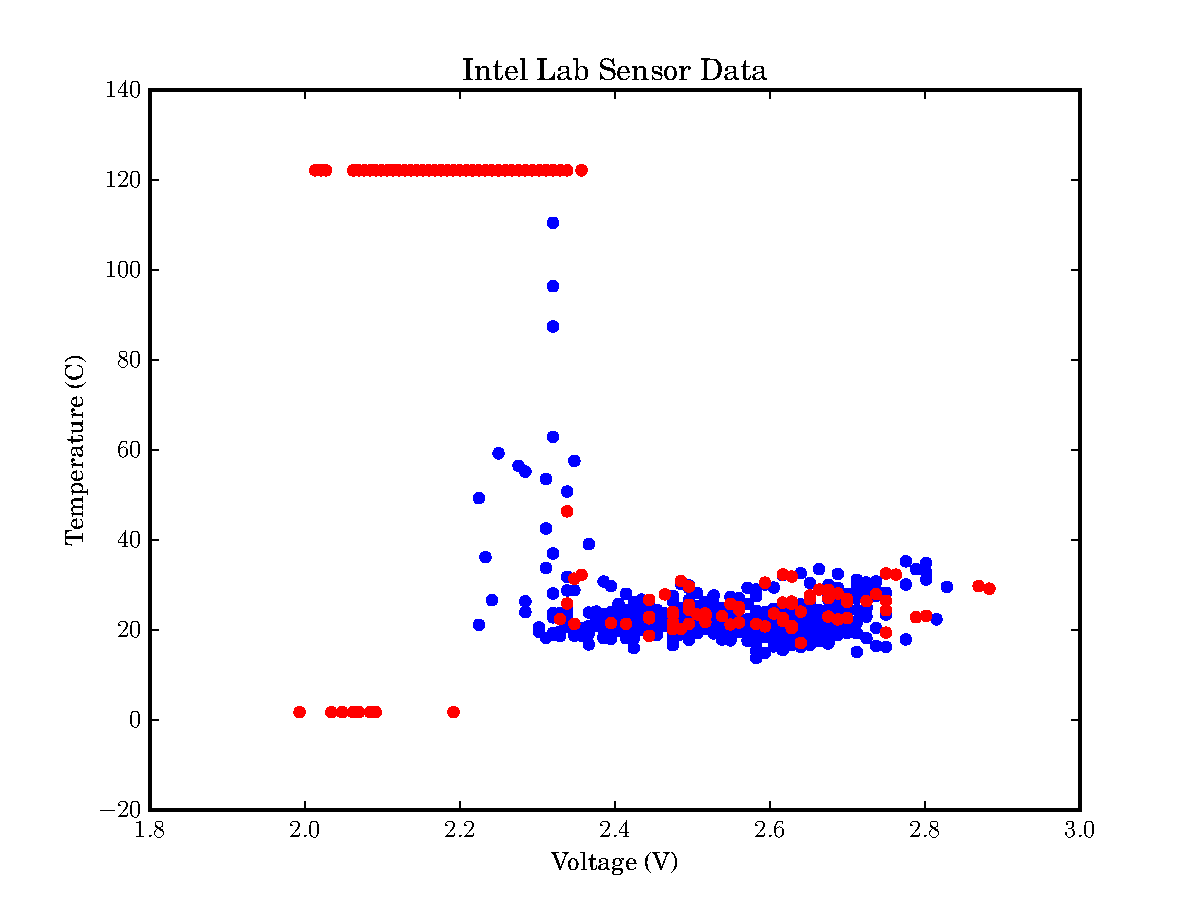
\includegraphics[width=0.45\textwidth]{../graphics/plots/sensors_gm.pdf}
\caption{Outliers from sensor data detected by a Gaussian model.}
\label{fig:sensors_1k_gm}
\end{figure}
\begin{figure}[h]
\centering
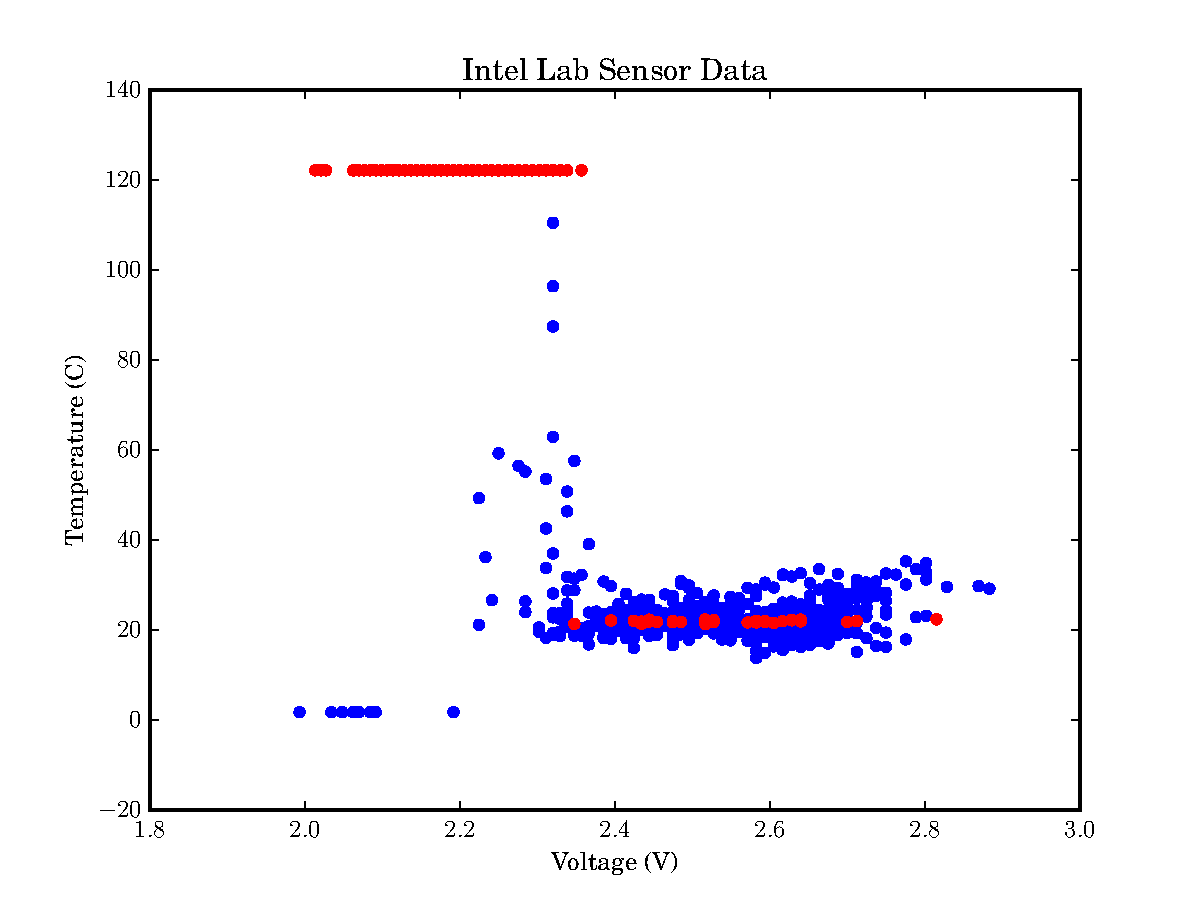
\includegraphics[width=0.45\textwidth]{../graphics/plots/sensors_mm.pdf}
\caption{Outliers from sensor data detected by a Mixture model.}
\label{fig:sensors_1k_mm}
\end{figure}

\subsection{Scalability}
\label{sec:performance-evaluation}

%We show in Figure~\ref{fig:scaling} how \dBoost/ scales as the amount of data used to build the models and to test on the models increases.
We measure the total runtime of our system, including the data modeling and outlier detection phases for the Simple Gaussian, Mixtures with 2 Gaussians, and Histograms. 
We used the Intel sensor data set from Section~\ref{sec:intel-lab-data-evaluation} to evaulate the Gaussian and Mixture models, and the CSAIL directory from Section~\ref{sec:csail-directory-evaluation} to evaluate the Histograms. 
We use random sampling to provide training sets of 1 thousand and 10 thousand elements from the Intel dataset to build the data models.
We test them on all 2+ million elements in the dataset.
To provide a more comprehensive study of the scalability of the Histogram model, we replicated the rows of the CSAIL directory to increase the training and test set sizes. 

In Figure~\ref{fig:scaling}, we show the runtime of our prototype. Each line shows a model trained with a different training set size. As shown in the figure, runtime scales linearly as the test set size increases.
Applying additional optimizations such as using a lower-level language or enabling parallism would improve runtime performance to production-ready levels. 

\begin{figure}
\centering
\paddedgraphics{../../graphics/scalability.pdf}
\caption{The scalability of the Gaussian and Mixture Models produced with different training sample sizes (listed next to the model in the legend) as the test set size increases.}
\label{fig:scaling}
\end{figure}

%\subsection{Presidential Campaign Finance}
\label{sec:presidential-campaign-evaluation}
\cite{PresCampaignData}

%\subsection{Mimic2}
\label{sec:mimic2-evaluation}


\section{Related Work}
\label{sec:related-work}

% Outlier Detection
There has been substantial research in how to build models to detect outliers \cite{Aggarwal2013}, including how to detect outliers in high-dimensional data by searching the subspaces of the data \cite{Zhang2004}\cite{Kriegel2009}.
However many of these algorithms are complex and can require substantial computation to determine whether a new data point lies outside the data.

Several algorithms exist in the data mining community to determine outliers when doing data analysis.
Local outlier factor measures the degree to which a data point is an outlier~\cite{Breunig2000}.
Other techniques include k-nearest neighbor~\cite{Ramaswamy2000} and cluster analysis.

% Outlier Detection Visualization
Research has been done to attempt to explain why outliers exist given properties of the original data~\cite{Wu}. Unlike our tool, Scorpion starts with user-defined outliers and works backwards to find potential explanations as to why the data points are outliers.

% Statistical methods
Statistical methods have been used to detect dependencies between columns of relational databases for the purpose of informing the query optimizer of potential data dependencies \cite{Ilyas2004}. These methods require only a small sample of the data to detect functional dependencies with high probability of correctness. The relatively low computation required by these algorithms makes them more amenable to detecting data anomalies in real time. However, these methods are better suited for numerical data~\cite{Hodge2004}

% Gaussian models
Gaussian Mixture Models have been used for outlier detection in multiple contexts~\cite{Lu2005,Roberts1994,Roberts1999}.

% Histograms
Histograms are used in conjunction with local outlier factors to detect outliers~\cite{Gebski2007,Sheng2007}, in cases of numerical or categorical data.

% String data
To the extent of our knowledge, the literature regarding outlier detection on non-numerical data is much less extensive. Some common approaches include identifying outliers using a similarity measure~\cite{Budalakoti2006}, Probabilistic Suffix Trees~\cite{Sun2006} and sequence alignment~\cite{Bouarfa2012}.

Some specialized work has focused on inferring domain-specific rules on highly specific data such as a sequence of UNIX commands~\cite{Lane1997a,Lane1997b}. By contrast, we take on a general-purpose approach that is capable of dealing with data as diverse as a set of names and office numbers to real-valued sensor data. Additionally, we analyze data without any additional information on its structure.

Overall, we differ from previous approaches in that we are capable of analyzing a very wide range of data and do not use predefined rules for outlier detection -- although adding user-defined rules is possible in our framework.

\begin{block}{\thighlight{Future work}}
\begin{itemize}
\item Extend framework to support run time queries
\item Provide more information on why model chose outliers
\item Implement additional models 
\end{itemize}

\end{block}

\section{Conclusion}
\label{sec:conclusion}

In this paper we presented \dBoost, a toolkit that leverages tuple expansion to detect outliers in both numerical and heterogeneous data sets. We demonstrated that well-known machine-learning strategies could be used to flag spurious numerical and to a lesser extent non-numerical data. We also demonstrated that simple correlation modeling is useful in inferring data dependencies and improving the accuracy of outlier detection procedures. We discussed histogram-based models, and showed that they provided a useful tool in analyzing mostly textual data.

We showed that our toolkit performs well on real-world problems, including identifying potentially wrong entries in a people directory and flagging erroneous values generated by faulty sensors. Our toolkit and its source code are available for public use under a permissive license, with the hope of allowing database users to formulate their own type-based rules and find discrepancies in their own data.

We believe that the preliminary results presented in this paper are promising, especially in the area of identifying outliers in heterogeneous data.


\section{Acknowledgments}
The authors would like to thank Eugene Wu (MIT CSAIL) for providing guidance on dataset selection, and Samuel Madden, Rebecca Taft, and Hongyu Yang (MIT CSAIL) for guidance and advice in the course of this project.


\balance
\bibliographystyle{abbrv}
\bibliography{paper.bib}


\clearpage
\pagebreak

\begin{figure}[h]
\centering
\includegraphics[width=0.45\textwidth,page=1]{../graphics/sensor-gaus-plots.pdf}
\caption{Simple Gaussian model}
\label{fig:sensors_gaus_1-5}
\end{figure}
\begin{figure}[h]
\centering
\includegraphics[width=0.45\textwidth,page=2]{../graphics/sensor-gaus-plots.pdf}
\caption{Simple Gaussian model}
\label{fig:sensors_gaus_1-5b}
\end{figure}

\begin{figure}[h]
\centering
\includegraphics[width=0.45\textwidth,page=1]{../graphics/sensor-plots.pdf}
\caption{Mixture model with 1 Gaussian}
\label{fig:sensors_1}
\end{figure}
\begin{figure}[h]
\centering
\includegraphics[width=0.45\textwidth,page=2]{../graphics/sensor-plots.pdf}
\caption{Mixture model with 1 Gaussian}
\label{fig:sensors_2}
\end{figure}
\begin{figure}[h]
\centering
\includegraphics[width=0.45\textwidth,page=3]{../graphics/sensor-plots.pdf}
\caption{Mixture model using no correlations}
\label{fig:sensors_nocorr}
\end{figure}
\begin{figure}[h]
\centering
\includegraphics[width=0.45\textwidth,page=1]{../graphics/sensor-mix-plots.pdf}
\caption{Mixture model with 2 Gaussians}
\label{fig:sensors_3}
\end{figure}
\begin{figure}[h]
\centering
\includegraphics[width=0.45\textwidth,page=2]{../graphics/sensor-mix-plots.pdf}
\caption{Mixture model with 2 Gaussians}
\label{fig:sensors_4}
\end{figure}
\begin{figure}[h]
\centering
\includegraphics[width=0.45\textwidth,page=1]{../graphics/lof-plots.pdf}
\caption{Local Outlier Factor for the $k$=2 nearest neighbors.}
\label{fig:lof_2}
\end{figure}
\begin{figure}[h]
\centering
\includegraphics[width=0.45\textwidth,page=2]{../graphics/lof-plots.pdf}
\caption{Local Outlier Factor for the $k$=10 nearest neighbors.}
\label{fig:lof_10}
\end{figure}


\end{document}
